\begin{frame}
\frametitle{Inscrição}
Caso não possua uma conta no URI, é possível iniciar a inscrição na página inicial do site.
 
\includegraphics[scale=.28]{uri/Imagens/01Login.png}
\end{frame}

\begin{frame}
 \frametitle{Cadastro}
 Insira as informações corretamente. E utilize um e-mail válido,
 pois será necessário confirmar a inscrição através dele.
 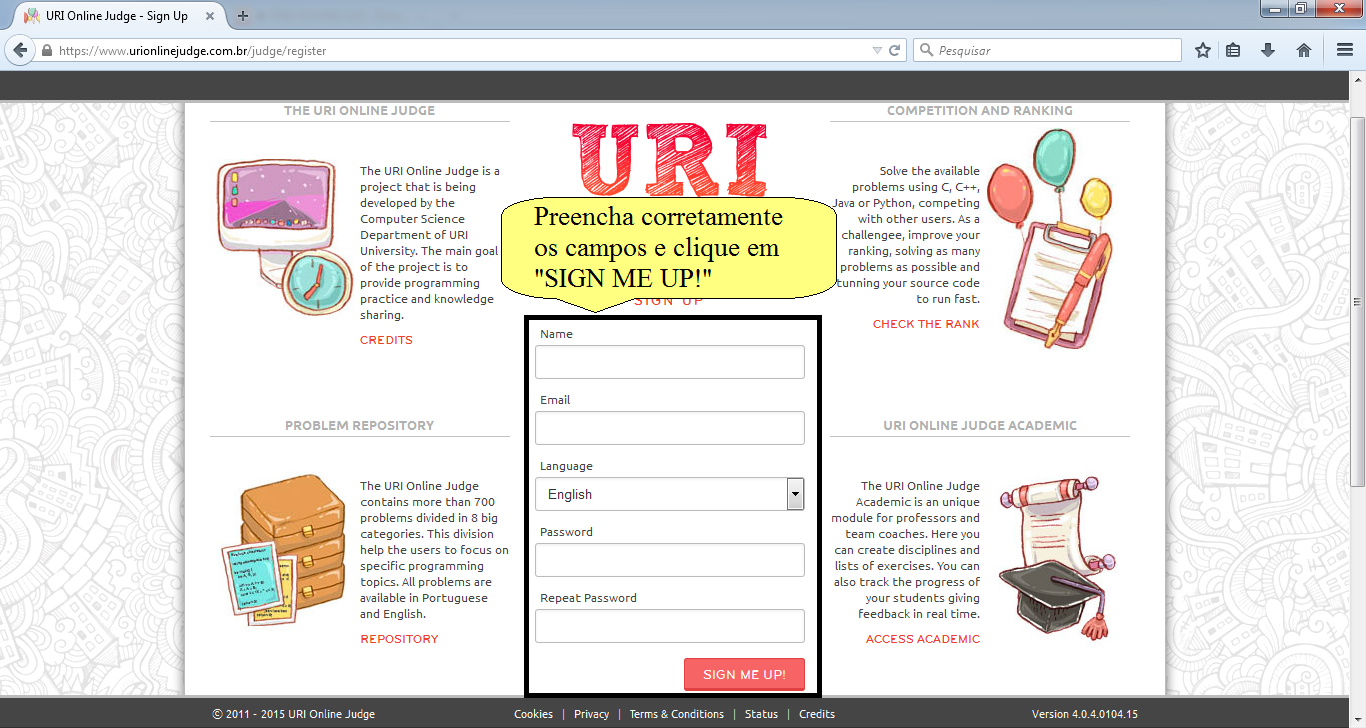
\includegraphics[scale=.28]{uri/Imagens/02Cadastro.png}
\end{frame}

\begin{frame}
  \frametitle{Confirmação}
Receberá um código de ativação no e-mail. Insira-o no campo como mostra a imagem
ou utilize o link que estará após o código de ativação no e-mail.
 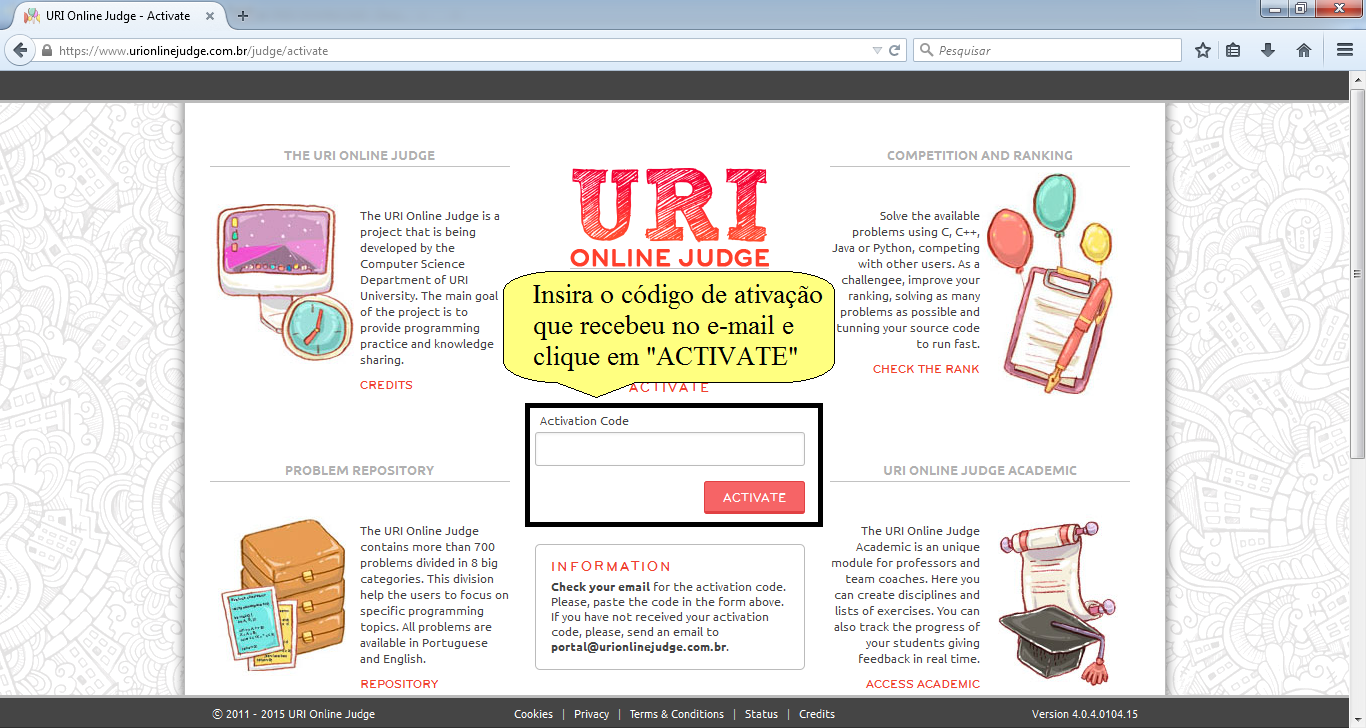
\includegraphics[scale=.28]{uri/Imagens/03Confirmacao.png}
\end{frame}

\begin{frame}
 \frametitle{Dashboard}
 Página inicial do usuário do URI.
 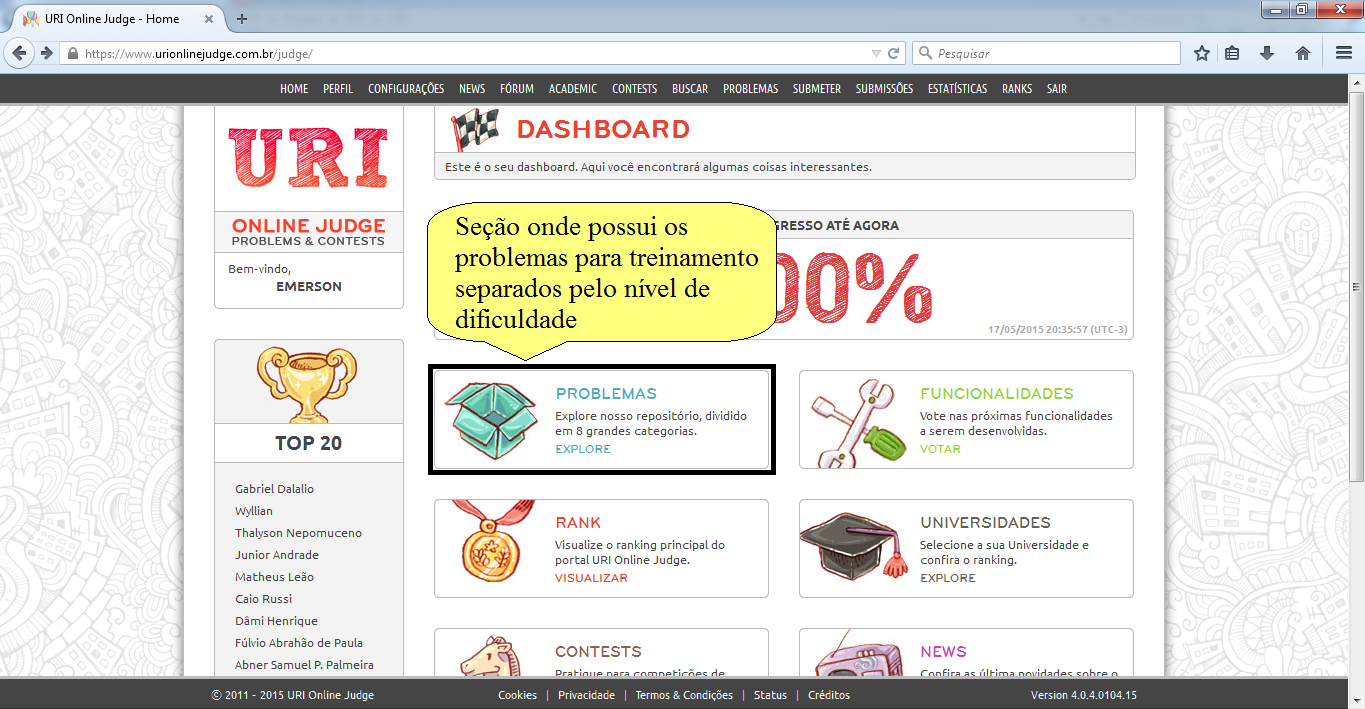
\includegraphics[scale=.28]{uri/Imagens/04Dashboard.png}
\end{frame}

\begin{frame}
 \frametitle{Categorias}
 Seção que possui os problemas separados por nível de conhecimento.
 Escolha uma seção e verá seus respectivos problemas.
 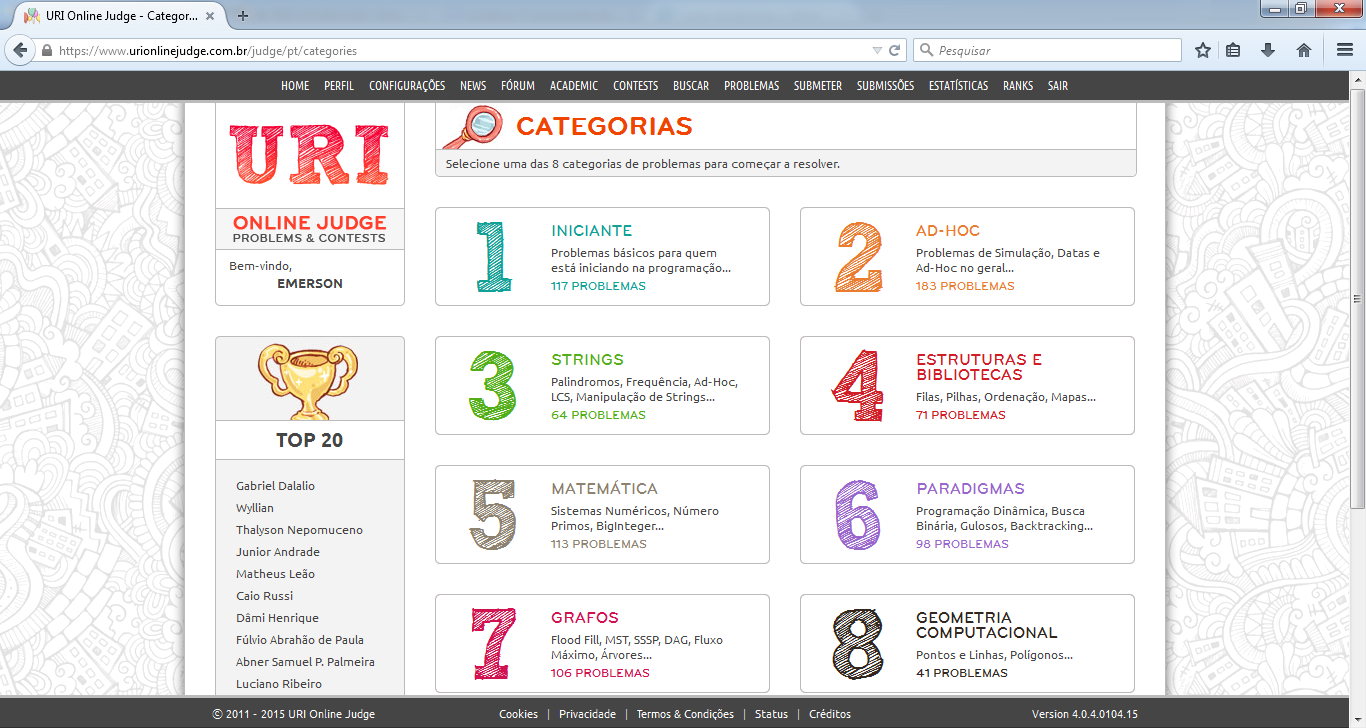
\includegraphics[scale=.28]{uri/Imagens/05Categorias.png}
\end{frame}

\begin{frame}
 \frametitle{Seção Iniciante}
 Ao selecionarmos a seção Iniciante, nos deparamos com os
 problemas para usuários iniciantes na programação.
 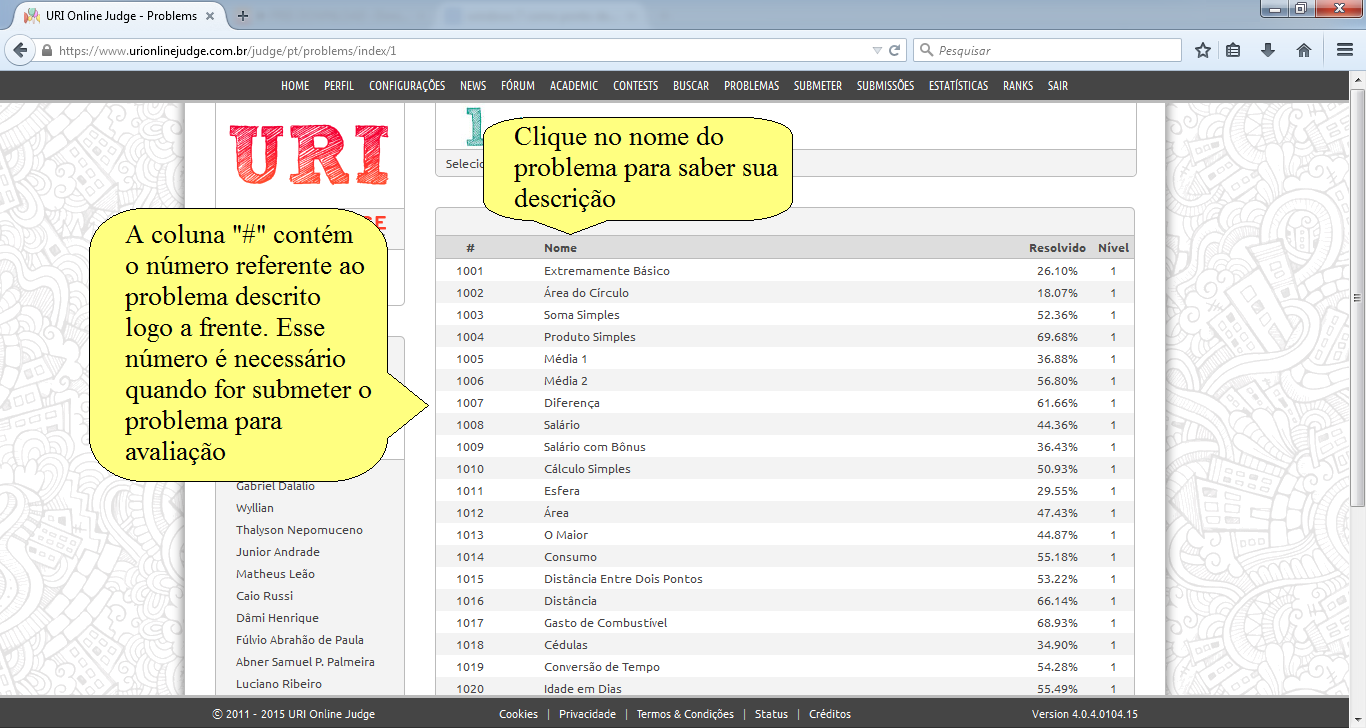
\includegraphics[scale=.28]{uri/Imagens/06Iniciante.png}
\end{frame}

\begin{frame}
 \frametitle{Descrição do problema}
 Após selecionarmos o problema Extremamente Básico, número 1001,
 é apresentado a descrição do problema e algumas informações.
 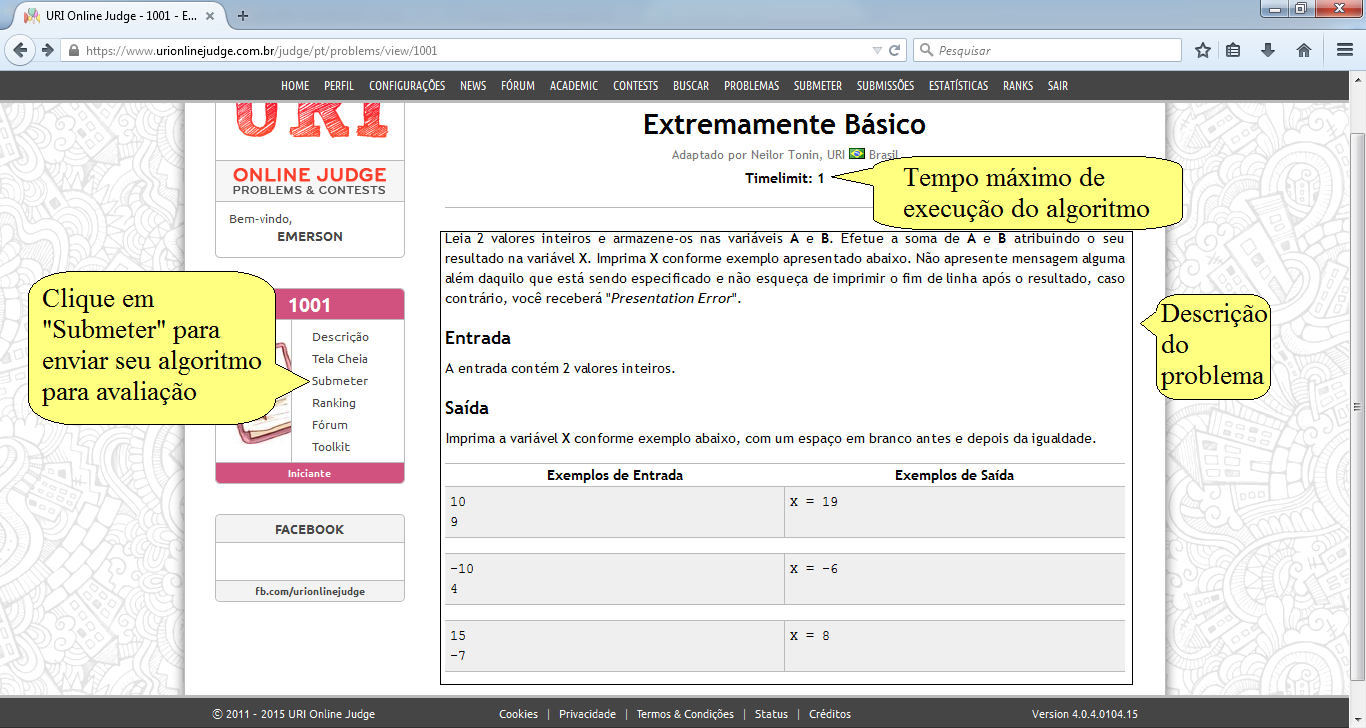
\includegraphics[scale=.28]{uri/Imagens/07DescricaoProblema.png}
\end{frame}

\begin{frame}
 \frametitle{Submeter}
 Ao construir e testar o algoritmo, deve-se submete-lo para validação.
 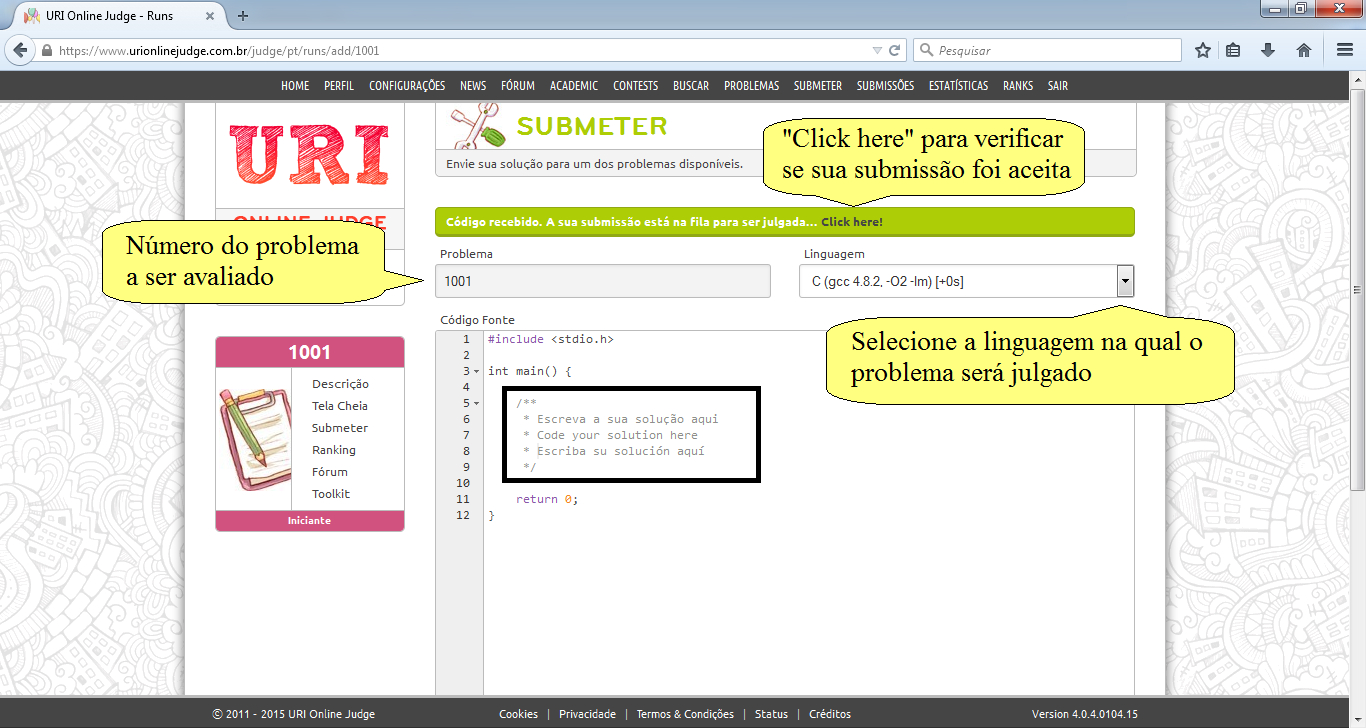
\includegraphics[scale=.28]{uri/Imagens/08Submeter.png}
\end{frame}

\begin{frame}
 \frametitle{Resultado}
 Após a submissão, verificará se seu algoritmo foi aceito ou não pelo URI.
 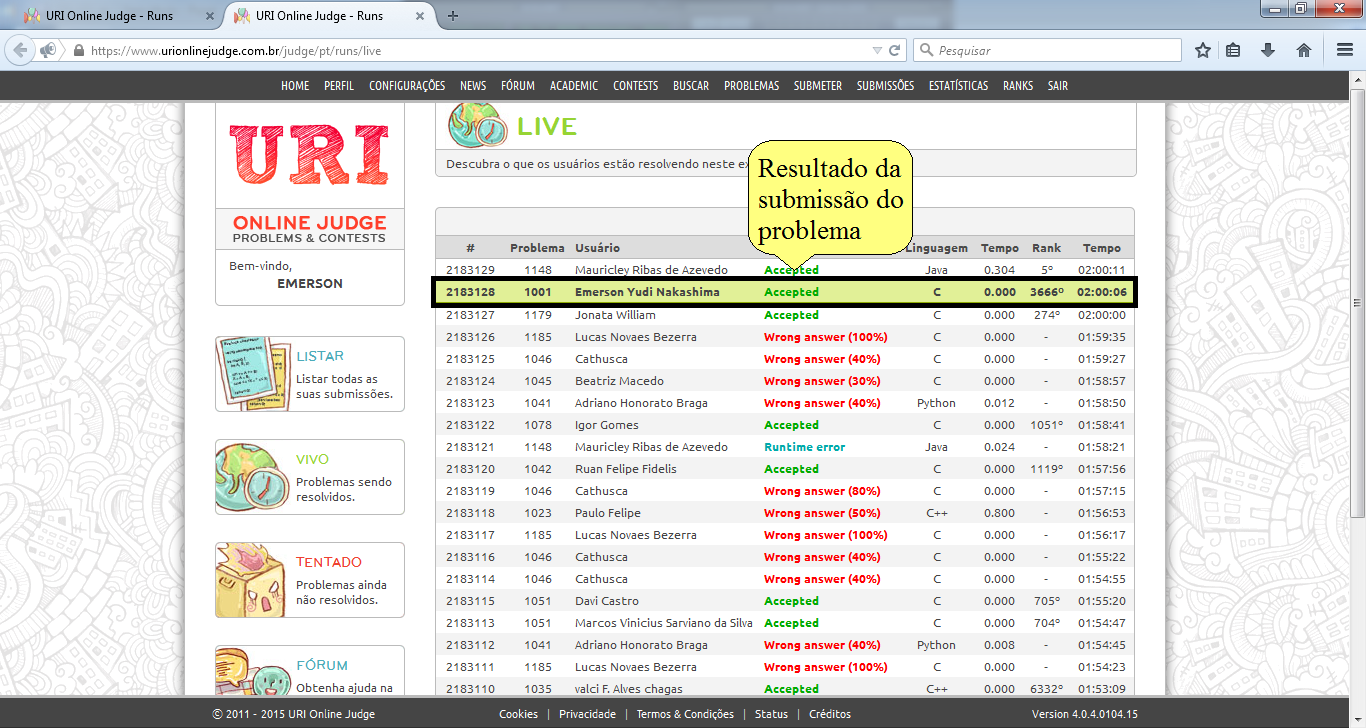
\includegraphics[scale=.28]{uri/Imagens/09Resultado.png}
\end{frame}